% kapitel2.tex



\newcounter{claims}
\newcounter{hypothesises}
\newtheorem{myclaim}[claims]{Scientific Claim}
\newtheorem{hypothesis}[hypothesises]{Hypothesis}

\chapter{Grundlagen}
\label{cha:grundlagen}

\section{Cartesian Genetic Programming}



\opensymdef
\newsym[lambda]{lam}{\lambda}
\newsym[my]{my}{\mu}
\closesymdef


Genetic Programming (GP), wie von Koza 
\cite{koza-90}\cite{koza:book}\cite{koza:gp2} 
verbreitet, nutzt Bäume zur Darstellung und Entwickelung von Programmen. Neue Generationen werden produziert, indem zufällig gewählte Teilbäume getauscht werden. Ursprünglich wurden Bäume als Datenstruktur gewählt, um Crossover zu unterschiedlich langer Genotypen zu ermöglichen. Später hat sich jedoch herausgestellt, dass Crossover nicht immer der beste genetische Operator ist um neue Generationen zu produzieren
\cite{luke:1997:ccmGP}\cite{luke:1998:rcxmGP}\cite{oai:generic.eprints.org:55371}.

Im Gegensatz zu GP benutzt CGP eine Liste aus Integern die auf gerichtete azyklische Graphen abgebildet werden. Durch eine fest bestimmte Anzahl an Knoten wird CGP vor 'aufblähen' geschützt, was ein Charakteristisches Problem von GP darstellt. Die Knoten sind in einem Gitter angeordnet und können nicht mit Knoten in der selben Spalte verbunden sein \ref{fig:cgpExample} Der gebräuchlichste Ansatz ist es, die Knoten in einer Reihe anzuordnen, sodass sich keine zwei Knoten in der selben Spalte befinden und für die Generierung der einer neuen Generation den (1+4) CGP Algorithmus () zu verwenden. Dieser nutzt das Individuum mit der geringsten Fitness und erzeugt aus diesem vier Nachkommen 
\cite{miller:2000:CGP}. 
Vor kurzem ist jedoch ein Paper erschienen, das sich mit einem Ansatz beschäftigt hat, bei dem ein rechteckiges Gitter und ein ($\mu$+$\lambda$) CGP Algorithmus verwendet werden\cite{conf/ki/KaufmannK17}. Während dieser bessere Resultate für boolsche und symbolische Regressionsfunktionen erzielt hat, wurde in dieser Arbeit der gebräuchliche (1+4) Ansatz verwendet, da dieser sich weiterhin für boolsche Benchmarks eignet.

\begin{algorithm}
\caption{(1+$\lambda$)-CGP Algorithmus}
\begin{algorithmic}[1]
\Procedure{(1+$\lambda$)-CGP}{}
   \State initialisiere($P$) \Comment{Initialisiere Eltern Individuum}
   \While{true}\Comment{Bis das Abbruchkriterium erfüllt ist}
      \State $Q \gets \textnormal{erzeugen(P)}$ \Comment{Erzeuge $\lambda$ Nachkommen durch Mutation}
      \State Evaluiere($Q$) \Comment{Evaluiere die Fitness der Nachkommen}
      \If {$Q$ \textit{das Abbruchkriterium erfüllt}}
              \State \textbf{return} $Q$
      \EndIf
      \If {\textit{mindestens ein Individuum von} $Q$ \textit{eine bessere Fitness hat als} $P$}
               \State $P \gets \textnormal{Q}$ \Comment{Ersetze das Eltern Inividuum durch den besten Nachkommen}
      \EndIf
   \EndWhile
\EndProcedure
\end{algorithmic}
\end{algorithm}



%BEGRIFFSDEFINITIONEN!!!: Fitness, Budget, mu, lambda
\begin{figure}
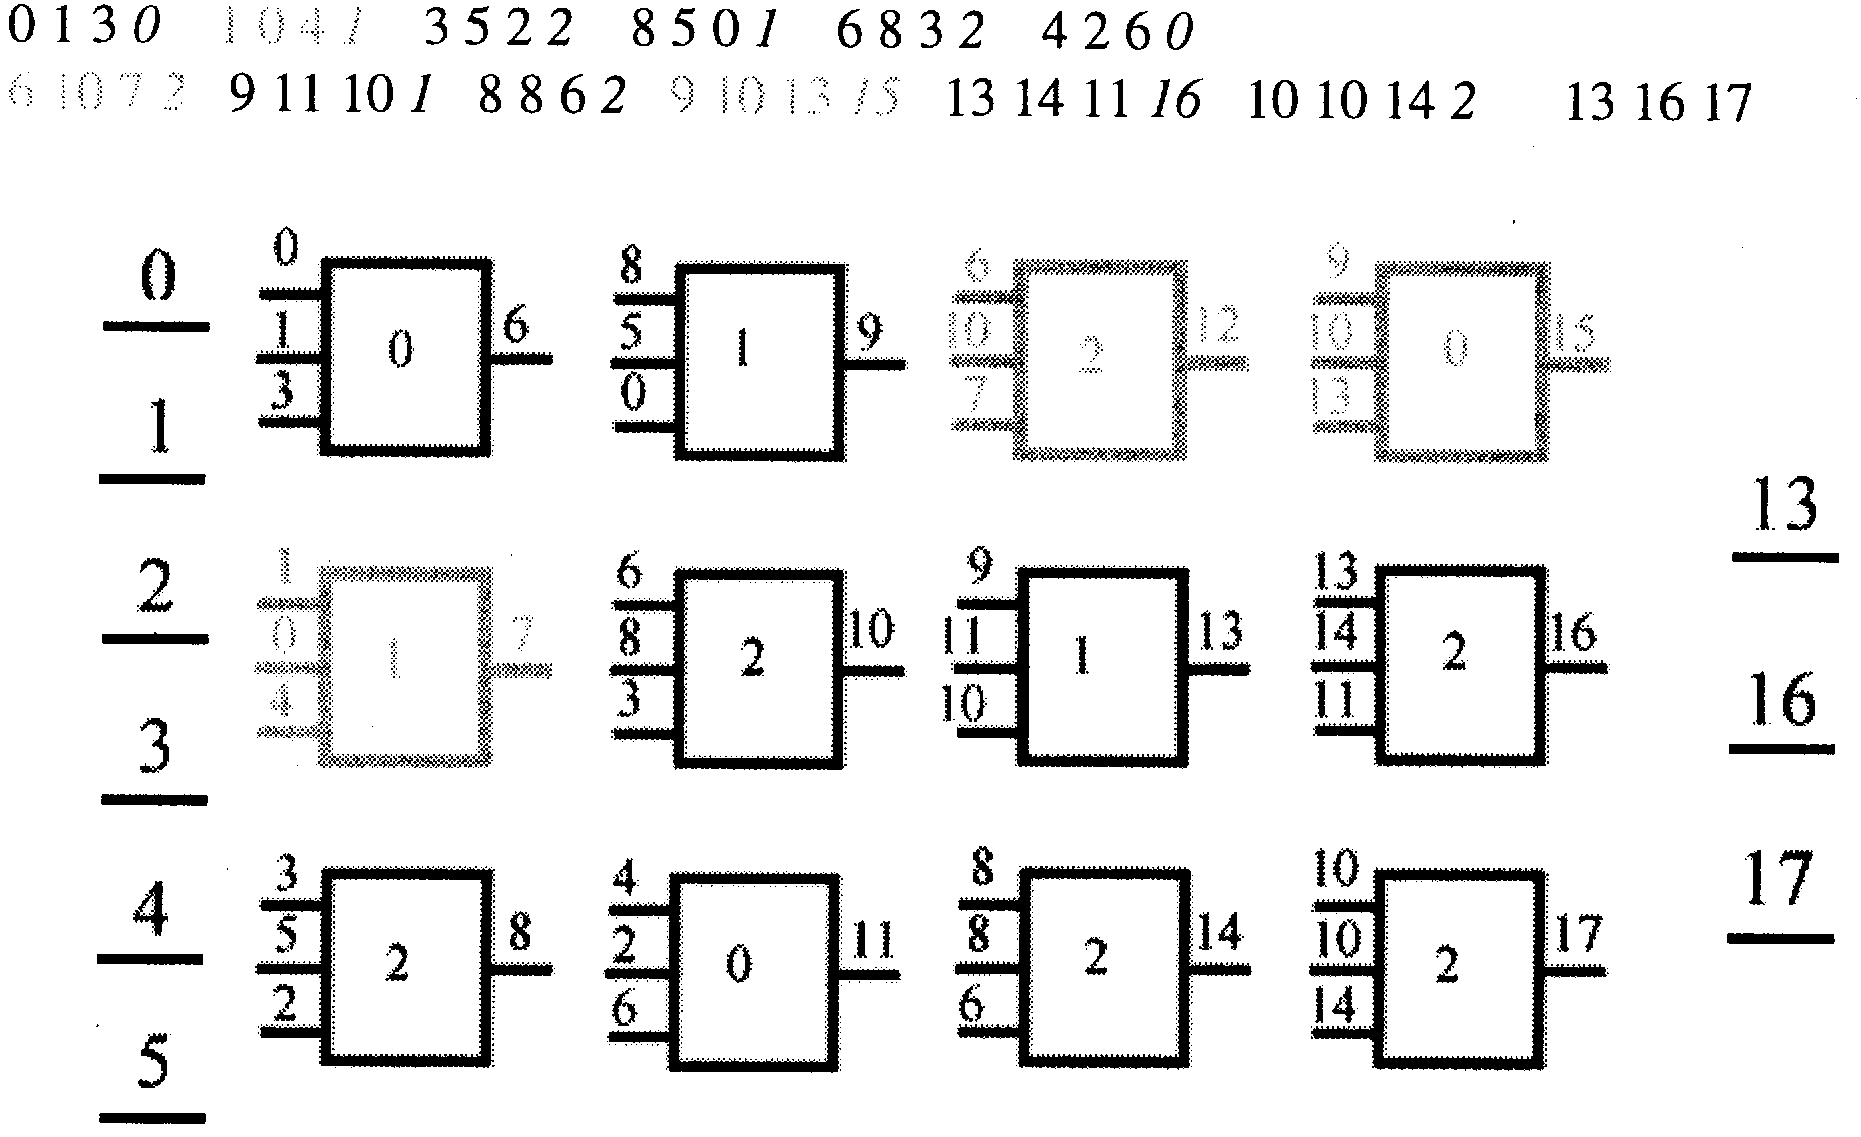
\includegraphics[scale=0.3]{cgpExample}
\caption[Beispielhafter Aufbau eines CGP]{}
\label{fig:cgpExample}
\end{figure}

\section{Mutationsalgorithmen}

Die folgenden Mutationsalgorithmen unterscheiden sich lediglich in der Auswahl der zu mutierenden Knoten. Sind ein oder mehrere Knoten ausgewählt, wird zufällig bestimmt ob sich eine der input Kanten ändert, oder ob die Funktion innerhalb des Knoten ausgetauscht wird.


\subsection{Traditioneller Mutationsalgorithmus}

Dies ist die Standardmethode für CGP. Es wird eine Mutationswahrscheinlichkeit angegeben (z.B. 0,01) und jeder Knoten hat diese Wahrscheinlichkeit zu mutieren. Somit kann es passieren, das die Hälfte der Knoten, oder gar kein Knoten mutiert. Da ein Großteil der Knoten nicht aktiv ist, passiert es bei einer geringen Mutationsrate häufig, das kein aktiver Knoten mutiert wird und sich somit die Fitness nicht ändert. Eine zu große Mutationsrate ist allerdings für viele Probleme ungeeignet, da das Zufallselement zu groß ist und eine Schrittweise Annäherung an das Ziel schwieriger wird.


\begin{algorithm}
\caption{traditioneller CGP Mutationsalgorithmus}
\begin{algorithmic}[1]
\Procedure{Mutationsalgorithmus für CGP}{}
   \State initialisiere($G$) \Comment{Initialisiere den Graph}
   \State initialisiere($W$) \Comment{Initialisiere die Mutationsrate}
   \ForAll{$E$ in $G$} \Comment{Für jede Kante und jeden Knoten im Graphen}
       \If {Wahr($W$)} \Comment{mit der Wahrscheinlichkeit $W$}
          \State \textnormal{gib $E$ einen zufälligen passenden Wert} \Comment{mutiere $E$}
      \EndIf
   \EndFor
\EndProcedure
\end{algorithmic}
\end{algorithm}

\subsection{Der Algorithmus single active gene mutation}

Bei der 'single active gene mutation' gibt es keine Mutationswahrscheinlichkeit. Stattdessen wird bei jedem Mutationsvorgang genau ein aktiver Knoten zufällig ausgewählt und dieser wie vorher beschrieben mutiert. Dabei ist es weiterhin möglich teile des Graphen zu aktivieren und zu deaktivieren, allerdings hat jede Mutation eine direkte Auswirkung auf das Ergebnis und somit auf die Fitness. Das soll das Problem der traditionellen Mutation lösen, bei der es sein kann, dass eine Mutation über mehrere Generationen keine Auswirkung auf die Fitness hat. Der Nachteil an 'single active gene mutation' ist, dass es nicht mit der Anzahl an Knoten im Graphen wächst. Ein mutierter Knoten pro Generation mag für einen Graphen mit 50 Knoten ausreichend sein, ist für einen Graphen mit 500 Knoten jedoch viel zu langsam. Außerdem wird sich 'single active gene mutation' wahrscheinlich nicht so gut auf Probleme anwenden lassen, die lokale Optima haben, da sich teile des Graphen zwar aktivieren und deaktivieren, jedoch nicht im inaktiven zustand verändern lassen.

Daher testen wir den Algorithmus auch mit mehreren mutierenden knoten. Dabei geben wir einen Parameter wie die Mutationswahrscheinlichkeit bei der traditionellen Mutation und in ganzen positiven Zahlen an.

\subsubsection{Der Algorithmus partial active gene mutation}

Bei der Mutation von Individuen kann es passieren das der aktive Teil des Graphen stark fluktuiert. Bei der traditionellen Mutationsmethode automatisch mehr aktive knoten mutiert werden, da die Wahrscheinlichkeit einen aktiven knoten zu treffen größer ist, wenn mehr vorhanden sind. Hierfür wird eine Variation der 'single active gene mutation' eingeführt, die 'partial active gene mutation'. Die 'partial active gene mutation' verhält sich wie die 'single active gene mutation', bestimmt allerdings für jedes Individuum die Mutationsrate neu um sie auf die Anzahl der aktiven knoten anzupassen. Dies geschieht mithilfe der derzeitigen Anzahl an aktiven Knoten und einem zu Beginn eingegebenen Mutationsbruchteil. Hierbei ist zu beachten, dass immer aufgerundet wird um zu verhindern das die Mutationsrate auf 0 sinkt wodurch wir feststecken würden. Ist der Bruchteil beispielsweise 0,02 und die Anzahl an aktiven Knoten 55, würden 2 aktive Knoten mutiert werden.



\section{Probleme}

Da 'Cartesian Genetic Programming' eignet sich besonders gut um boolsche Probleme \cite{miller:1999:ACGP} und Probleme mit mehreren Outputs zu lösen. Daher nutzen wir zwei boolsche Probleme um den Mutationsalgorithmus zu testen, von denen eines mehrere Ausgaben und das andere eine Ausgabe hat.

\subsection{Parität}

%formeller/mathematischer ausdrücken
Als boolsches Problem mit einer Ausgabe, verwenden wir das Paritätsproblem. Hierbei erhält das CGP eine Bitfolge und gibt TRUE aus, falls die Parität der Bitfolge gerade ist, also falls sich eine gerade Anzahl an Einsen in der Bitfolge befinden, andernfalls gibt das Programm FALSE aus. Das CGP hat also X Inputknoten und einen Outputknoten, wobei X die Länge der Bitfolge ist. Dieses Problem lässt sich in unterschiedlichem Umfang anwenden, da mit steigender Länge des Eingabebits die Anzahl der Generationen bis das CGP das Problem lösen kann zunimmt. Wir verwenden unterschiedliche Varianten des Paritätsproblems, mit einer Eingabe von 4, 5, 6 und 7 Bits. Mehr erfahren wir später.


\subsection{3-Bit-Multiplizierer}

%Abbildung oder definition für 3bit multiplier
Das 3-Bit-Multiplizierer Problem (ebenfalls boolsches Problem) ist besonders spannend, da sich die Graphen basierte Struktur des CGP anbietet Schaltkreise darzustellen. Hierbei versuchen wir aus dem CGP einen 3-Bit-Multiplizierer zu machen. Wir brauchen also 2 Bitfolgen die jeweils 3 Bits lang sind. Mit 3 Bits lässt sich 7 als größte Zahl darstellen. sieben mal sieben ist gleich 49, welche sich mit 6 Bits darstellen lässt, also brauchen wir 6 Bits für die Ausgabe. Unser Graph braucht also 6 Inputknoten und 6 Ouputknoten.

\chapter{Versuche}


\section{Versuchskonfiguration}

Zur Versuchsdurchführung nutzen wir zwei boolsche Probleme genutzt, 3-Bit-Multiplizierer und Parität, wobei wir die Varianten Parität 4, Parität 5, Parität 6 und Parität 7 verwenden. Um zu bewerten, wie Effizient die Mutationsalgorithmen arbeiten, lassen wir uns die Anzahl der Generationen ausgeben, bis ein Graph gefunden wurde, der das Problem löst. Das Ziel ist es die Anzahl der Generationen zu verringern, da mehr Generationen mehr Auswertungen der Graphen bedeuten was wiederum Rechenzeit in Anspruch nimmt. Verglichen werden der traditionelle Mutationsalgorithmus, 'single active gene mutation', sowie 'partial active gene mutation'.

Als Ursprungspopulation werden zufällig generierte Graphen genutzt. Eine neue Generation wird nach dem (1 + 4) CGP Algorithmus generiert. Dabei wird das Individuum mit der niedrigsten Fitness ausgewählt und viermal mutiert, somit besteht eine Generation immer aus einem Individuum aus der vorherigen Generation und 4 Nachkommen von diesem. Bei der Auswahl eines Individuums werden bei gleicher Fitness Nachkommen bevorzugt.

\begin{hypothesis}
Der 'single active gene mutation' Algorithmus benötigt weniger Generationen um Probleme aus allen Bereichen zu lösen als der traditionelle Wahrscheinlichkeitsbasierte Mutationsalgorithmus.
\end{hypothesis}

Um die Hypothese zu testen, lassen wir die Algorithmen auf den jeweiligen Probleme mit 50, 100, 200, 500 und 1000 Knoten 60 mal laufen, mit Ausnahme von Parität 7, welches wir nur mit 200 Knoten und 30 Durchläufen testen. Da einige Durchläufe nicht innerhalb von 9999999 Generationen fertig geworden sind, machen wir eine zweite Reihe von Versuchen. Dafür verwenden wir die Konfigurationen der Versuche, die vorher mindestens ein drittel der Durchläufe nicht innerhalb der 9999999 Generationen beenden konnten. Hierbei benutzen wir allerdings nur ein Budget von 999999 Generationen und lassen uns, falls dieses erreicht wird die Fitness des besten Individuums, ausgeben.
\begin{table}[!ht]
\centering 
\caption{Konfiguration der Versuche für das Paritätsproblem mit 4, 5, 6 und 7 Eingabeknoten.}
\scalebox{0.82}{
\begin{tabular}{|l|l||r|r|r|}
\hline
\scriptsize \textbf{Problem} & \scriptsize \textbf{Algorithmus} & \scriptsize \textbf{Mutations} & \scriptsize \textbf{Anzahl der} & \scriptsize \textbf{Durchläufe} \\
& & \scriptsize  \textbf{rate} & \scriptsize  \textbf{Knoten} &  \\ \hline


  \multirow{ 3 }{*}{Parität 4 /  5 /  6}  
   & traditionelle Mutation & 0.04 & 50 - 1000* & 60 \\
   & single active gene mutation & 1/2/3/4 & 50 - 1000* & 60 \\ 
   & partial active gene mutation & 0.01/0.03 & 50 - 1000* & 60 \\
      \hline
   
  \multirow{ 3 }{*}{Parität 7}  
   & traditionelle Mutation & 0.03 & 200 & 30 \\
   & single active gene mutation & 1/2/3/4 & 200 & 30 \\ 
   & partial active gene mutation & 0.01/0.03 & 200 & 30 \\
      \hline
   
  \multirow{ 3 }{*}{3-Bit-Multiplizierer}  
   & traditionelle Mutation & 0.01 & 50 - 1000* & 60 \\
   & single active gene mutation & 1/2/3/4 & 50 - 1000* & 60 \\ 
   & partial active gene mutation & 0.01/0.03 & 50 - 1000* & 60 \\
      \hline
      \multicolumn{4}{l}{\textsuperscript{}\small{\{50, 100, 200, 500, 1000\}. }} \\
\end{tabular}
}
\label{table_meta3}
\end{table}


Die Implementation ist in Java, mithilfe des ECJ Evolutionary Computation Research System und der zugehörigen CGP Erweiterung geschehen. Die Versuche wurden auf dem Batchsystem des LS 11 der Fakultät Informatik an der TU Dortmund ausgeführt. Für die zweite Reihe von Versuchen wurde ein Computer mit folgender Hardware genutzt:  AMD Ryzen 5 1500X Quad-Core Processor, 3.5 GHz, 18 MB cache per core; 8GB RAM DDR4@2133 MHz


\section{Ergebnisse für das Paritätsproblem}

Obwohl viele unterschiedliche Variablen gesetzt wurden, führen alle Versuche für das Paritätsproblem zu einem sehr ähnlich Ergebnis. Wie in Tabelle 3.2 zu sehen ist, schneidet die 'single active gene mutation' wesentlich besser ab, die Generationenanzahl des traditionellen Algorithmus sind im Median doppelt bis fasst viermal so groß. Bezüglich der Mutationsrate ist aber kein Muster zu erkennen. Weder ist eine bestimmte Mutationsrate besonders erfolgreich, noch scheint es sich proportional oder antiproportional zu der Knotenanzahl zu verhalten. Während die 'partial active gene mutation' zwar ebenfalls weniger Generationen benötigt als der traditionelle Algorithmus, verhält er sich dennoch für die meisten versuche nicht so effizient wie die 'single active gene mutation'. Allerdings scheint hier die niedrigere Mutationsrate bessere Ergebnisse zu erzielen.




\begin{table}[!ht]
\centering 
\caption{Resultate der Versuchsreihe für das Paritätsproblem mit vier Eingabeknoten.}
\scalebox{0.82}{
\begin{tabular}{ |l|l|r||r|r|r|r|r|}
\hline
\scriptsize \textbf{Knoten} & \scriptsize \textbf{Algorithmus} & \scriptsize \textbf{Mutations} & \scriptsize \textbf{min} & \scriptsize \textbf{unteres} & \scriptsize \textbf{Median} & \scriptsize \textbf{oberes} & \scriptsize \textbf{max} \\
& & \scriptsize  \textbf{rate} & \scriptsize  \textbf{}  & \scriptsize \textbf{quartil}& \scriptsize  \textbf{}& \scriptsize  \textbf{quartil}& \scriptsize  \textbf{} \\ \hline


  \multirow{ 7 }{*}{50}  
   & traditionelle Mutation & 0.04 & 2502 & 17343.25 & 26748.50 & 45067.50 & 131069 \\
   & single active gene mutation & 1 & 2198 & 7322.75 & 13181.00 & 21272.50 & 41109 \\ 
   & single active gene mutation & 2 & 1092 & 9059.75 & 12741.00 & 22042.50 & 68551 \\
   & single active gene mutation & 3 & 1413 & 5637.25 & 9359.50 & 16637.00 & 149940 \\
   & single active gene mutation & 4 & 3042 & 7411.75 & 13443.50 & 23293.00 & 70787 \\
   & partial active gene mutation & 0.01 & 2155 & 9312.25 & 16398.50 & 21842.00 & 84162 \\
   & partial active gene mutation & 0.03 & 2956 & 8523.75 & 16926.00 & 27037.50 & 166452 \\
      \hline
   
  \multirow{ 7 }{*}{100}  
   & traditionelle Mutation & 0.04 & 3472 & 11533.50 & 17073.00 & 29156.75 & 66681 \\
   & single active gene mutation & 1 & 2211 & 4268.25 & 6837.50 & 11410.75 & 36836 \\ 
   & single active gene mutation & 2 & 2391 & 4149.75 & 7614.00 & 12833.25 & 49861 \\
   & single active gene mutation & 3 & 932 & 4122.25 & 7574.50 & 14948.75 & 39941 \\
   & single active gene mutation & 4 & 1795 & 6201.00 & 9558.00 & 14735.25 & 72646 \\
   & partial active gene mutation & 0.01 & 1302 & 6082.25 & 9521.00 & 15979.50 & 61606 \\
   & partial active gene mutation & 0.03 & 1612 & 6426.00 & 10895.5 & 16346.00 & 29200 \\
      \hline
  
  \multirow{ 7 }{*}{200}
   & traditionelle Mutation & 0.04 & 4464 & 9778.00 & 15021.50 & 20934.50 & 49779 \\
   & single active gene mutation & 1 &  558 & 2881.75 & 5506.00 & 8266.75 & 20606 \\ 
   & single active gene mutation & 2 & 434 & 3324.25 & 4915.00 & 9501.00 & 33647 \\
   & single active gene mutation & 3 & 515 & 3914.75 & 5686.00 & 9553.75 & 28427 \\
   & single active gene mutation & 4 & 1425 & 3329.00 & 5889.50 & 9790.00 & 25937 \\
   & partial active gene mutation & 0.01 & 936 & 5002.75 & 7904.00 & 13101.25 & 46147 \\
   & partial active gene mutation & 0.03 & 1468 & 5418.00 & 7435.50 & 13910.50 & 36396 \\
      \hline
   
  \multirow{ 7 }{*}{500}
   & traditionelle Mutation & 0.04 & 1972 & 8576.00 & 12490.00 & 19928.25 & 98274 \\
   & single active gene mutation & 1 &  663 & 2622.75 & 4258.00 & 6622.50 & 18702 \\ 
   & single active gene mutation & 2 & 676 & 2209.75 & 3905.00 & 6450.50 & 16996 \\
   & single active gene mutation & 3 & 491 & 2729.75 & 4196.50 & 6933.00 & 16982 \\
   & single active gene mutation & 4 & 567 & 2687.25 & 3752.00 & 6323.75 & 16082 \\
   & partial active gene mutation & 0.01 & 850 & 3239.75 & 5362.50 & 9609.75 & 24918 \\
   & partial active gene mutation & 0.03 & 805 & 4159.75 & 7377.00 & 14285.75 & 27501 \\
      \hline
    
  \multirow{ 7 }{*}{1000} 
   & traditionelle Mutation & 0.04 & 1450 & 5813.00 & 11499.00 & 19757.25 & 67705 \\
   & single active gene mutation & 1 &  663 & 1764.50 & 3566.00 & 7230.25 & 22658 \\ 
   & single active gene mutation & 2 & 974 & 2540.25 & 3740.00 & 5920.00 & 30927 \\
   & single active gene mutation & 3 & 755 & 2298.50 & 3238.50 & 5131.25 & 14659 \\
   & single active gene mutation & 4 & 758 & 2298.50 & 3806.00 & 5639.00 & 19191 \\
   & partial active gene mutation & 0.01 & 1300 & 3718.00 & 6019.00 & 8050.25 & 15084 \\
   & partial active gene mutation & 0.03 & 903 & 3732.00 & 6051.50 & 10089.75 & 27084 \\
      \hline

\end{tabular}
}
\label{table_meta3}
\end{table}


\begin{table}[!ht]
\centering 
\caption{Resultate der Versuchsreihe für das Paritätsproblem mit fünf Eingabeknoten.}
\scalebox{0.82}{
\begin{tabular}{ |l|l|r||r|r|r|r|r|}
\hline
\scriptsize \textbf{Knoten} & \scriptsize \textbf{Algorithmus} & \scriptsize \textbf{Mutations} & \scriptsize \textbf{min} & \scriptsize \textbf{unteres} & \scriptsize \textbf{Median} & \scriptsize \textbf{oberes} & \scriptsize \textbf{max} \\
& & \scriptsize  \textbf{rate} & \scriptsize  \textbf{}  & \scriptsize \textbf{quartil}& \scriptsize  \textbf{}& \scriptsize  \textbf{quartil}& \scriptsize  \textbf{} \\ \hline


  \multirow{ 7 }{*}{50}  
   & traditionelle Mutation & 0.04 & 14420 & 79036.50 & 131375.00 & 234888.50 & 883025 \\
   & single active gene mutation & 1 & 7821 & 26325.25 & 52114.00 & 89874.75 & 229080 \\ 
   & single active gene mutation & 2 & 8108 & 33631.00 & 52251.00 & 78270.00 & 309113 \\
   & single active gene mutation & 3 & 3617 & 32635.50 & 56789.50 & 92668.75 & 247193 \\
   & single active gene mutation & 4 & 5074 & 33785.25 & 56548.00 & 80488.50 & 345667 \\
   & partial active gene mutation & 0.01 & 14255 & 50575.50 & 76934.00 & 113499.50 & 342851 \\
   & partial active gene mutation & 0.03 & 9002 & 57307.50 & 94587.00 & 190504.50 & 539069 \\
      \hline
   
  \multirow{ 7 }{*}{100}  
   & traditionelle Mutation & 0.04 & 10050 & 43432.00 & 64054.50 & 123934.20 & 762828 \\
   & single active gene mutation & 1 & 8448 & 24485.75 & 32460.50 & 48301.25 & 121953 \\ 
   & single active gene mutation & 2 & 2347 & 26255.25 & 34373.00 & 52626.50 & 218644 \\
   & single active gene mutation & 3 & 3283 & 19364.50 & 35372.50 & 57732.50 & 159130 \\
   & single active gene mutation & 4 & 3998 & 14561.25 & 23677.00 & 49354.75 & 312394 \\
   & partial active gene mutation & 0.01 & 4835 & 28415.00 & 53055.50 &  71386.00 & 214309 \\
   & partial active gene mutation & 0.03 & 9735 & 36568.75 & 68544.00 & 123667.00 & 287047 \\
      \hline
  
  \multirow{ 7 }{*}{200}
   & traditionelle Mutation & 0.04 & 18457 & 44458.75 & 63742.00 & 90995.50 & 326978.00 \\
   & single active gene mutation & 1 & 3376 & 16104.25 & 22043.00 & 34467.50 & 89430.00 \\ 
   & single active gene mutation & 2 & 2614 & 13555.50 & 20917.00 & 32370.25 & 104281.00 \\
   & single active gene mutation & 3 & 3451 & 14334.25 & 21260.00 & 30351.00 & 76023.00 \\
   & single active gene mutation & 4 & 3496 & 13844.50 & 21860.00 & 37714.50 & 122635 \\
   & partial active gene mutation & 0.01 & 4123 & 18474.00 & 33972.50 & 58223.00 & 196569 \\
   & partial active gene mutation & 0.03 & 7590 & 35797.50 & 49306.00 & 74395.25 & 276860 \\
      \hline
   
  \multirow{ 7 }{*}{500}
   & traditionelle Mutation & 0.04 & 16086 & 47853.00 & 70756.00 & 100628.80 & 276977 \\
   & single active gene mutation & 1 & 4496 & 8806.75 & 14873.00 & 25155.25 & 64016 \\ 
   & single active gene mutation & 2 & 3076 & 9335.75 & 13591.00 & 23677.25 & 88436 \\
   & single active gene mutation & 3 & 3527 & 11014.50 & 18751.50 & 29077.50 & 64083 \\
   & single active gene mutation & 4 & 2747 & 8852.25 & 14934.00 & 24295.00 & 76286 \\
   & partial active gene mutation & 0.01 & 4283 & 15321.00 & 29576.00 & 50473.50 & 108426 \\
   & partial active gene mutation & 0.03 & 10151 & 24992.25 & 43397.00 & 74513.75 & 206447 \\
      \hline
    
  \multirow{ 7 }{*}{1000} 
   & traditionelle Mutation & 0.04 & 13028 & 54985.00 & 105839.00 & 163160.80 & 646226 \\
   & single active gene mutation & 1 & 2480 & 9096.50 & 12259.50 & 20135.75 & 73618 \\ 
   & single active gene mutation & 2 & 2021 & 7196.75 & 11434.50 & 19332.00 & 43256 \\
   & single active gene mutation & 3 & 4665 & 9066.75 & 14160.00 & 21748.50 & 47843 \\
   & single active gene mutation & 4 & 3190 & 8239.25 & 13942.00 & 20980.00 & 97955 \\
   & partial active gene mutation & 0.01 & 6551 & 16809.75 & 26701.50 & 39634.25 & 121868 \\
   & partial active gene mutation & 0.03 & 10244 & 32186.50 & 46186.00 & 83316.00 & 192520 \\
      \hline

\end{tabular}
}
\label{table_meta3}
\end{table}


\begin{table}[!ht]
\centering 
\caption{Resultate der Versuchsreihe für das Paritätsproblem mit sechs Eingabeknoten.}
\scalebox{0.82}{
\begin{tabular}{ |l|l|r||r|r|r|r|r|}
\hline
\scriptsize \textbf{Knoten} & \scriptsize \textbf{Algorithmus} & \scriptsize \textbf{Mutations} & \scriptsize \textbf{min} & \scriptsize \textbf{unteres} & \scriptsize \textbf{Median} & \scriptsize \textbf{oberes} & \scriptsize \textbf{max} \\
& & \scriptsize  \textbf{rate} & \scriptsize  \textbf{}  & \scriptsize \textbf{quartil}& \scriptsize  \textbf{}& \scriptsize  \textbf{quartil}& \scriptsize  \textbf{} \\ \hline


  \multirow{ 7 }{*}{50}  
   & traditionelle Mutation & 0.04 & 162550 & 401197.00 & 698242.50 & 1232138.50 & 6181056 \\
   & single active gene mutation & 1 & 20973 & 104689.20 & 161482.00 & 257618.00 & 716348 \\ 
   & single active gene mutation & 2 & 37665 & 124028.00 & 186777.50 & 399768.80 & 2320344 \\
   & single active gene mutation & 3 & 20791 & 138583.80 & 212872.50 & 301570.20 & 621723 \\
   & single active gene mutation & 4 & 23834 & 106537.80 &  215655.00 & 321488.50 & 1799202 \\
   & partial active gene mutation & 0.01 & 35055 & 164097.20 & 268906.00 & 492241.00 & 2169102 \\
   & partial active gene mutation & 0.03 & 92581 & 220825.50 & 426964.50 & 587954.00 & 1038598 \\
      \hline
   
  \multirow{ 7 }{*}{100}  
   & traditionelle Mutation & 0.04 & 82090 & 240667.00 & 392821.00 & 628589.20 & 2134465 \\
   & single active gene mutation & 1 & 22908 & 70538.00 & 104221.50 & 148968.00 & 482618 \\ 
   & single active gene mutation & 2 & 23606 & 54632.00 & 96516.00 & 160370.20 & 648324 \\
   & single active gene mutation & 3 & 29737 & 79339.00 & 128264.50 & 213873.80 & 533257 \\
   & single active gene mutation & 4 & 10963 & 58809.00 & 118958.50 & 181560.20 & 638987 \\
   & partial active gene mutation & 0.01 & 10963 & 58809.00 & 118958.50 & 181560.20 & 638987 \\
   & partial active gene mutation & 0.03 & 33518 & 124603.50 & 250020.50 & 387999.80 & 1250051 \\
      \hline
  
  \multirow{ 7 }{*}{200}
   & traditionelle Mutation & 0.04 & 63125 & 177016.80 & 379967.00 & 538201.00 & 1633500 \\
   & single active gene mutation & 1 & 29949 & 55460.50 & 87846.00 & 126130.20 & 325626.0 \\ 
   & single active gene mutation & 2 & 12803 & 35799.00 & 48643.00 & 77012.00 & 223461 \\
   & single active gene mutation & 3 & 4565 & 34661.25 & 64311.00 & 104867.75 & 451110.00 \\
   & single active gene mutation & 4 & 14800 & 39245.00 & 58058.50 & 107041.80 & 384339.0 \\
   & partial active gene mutation & 0.01 & 16208 & 91772.00 & 151467.50 & 215949.0 & 1264939.0 \\
   & partial active gene mutation & 0.03 & 40233 & 124840.80 & 211505.00 & 351461.2 & 1052083.0 \\
      \hline
   
  \multirow{ 7 }{*}{500}
   & traditionelle Mutation & 0.04 & 39567 & 235274.80 & 336767.50 & 558199.20 & 1898404 \\
   & single active gene mutation & 1 & 2367 & 26372.00 & 47225.50 & 62354.75 & 205153 \\ 
   & single active gene mutation & 2 & 6901 & 32062.75 & 46302.00 & 67944.00 & 166649 \\
   & single active gene mutation & 3 & 7719 & 27645.75 & 48333.50 & 62789.50 & 259724 \\
   & single active gene mutation & 4 & 6557 & 22584.25 & 36786.50 & 63866.25 & 169185 \\
   & partial active gene mutation & 0.01 & 13083 & 83752.75 & 131489.00 & 186689.75 & 543667 \\
   & partial active gene mutation & 0.03 & 44180 & 101847.80 & 181634.50 & 239310.80 & 699155 \\
      \hline
    
  \multirow{ 7 }{*}{1000} 
   & traditionelle Mutation & 0.04 & 55929 & 196029.00 & 392648.00 & 755801.50 & 3791696 \\
   & single active gene mutation & 1 & 6859 & 24890.75 & 48989.00 & 84916.00 & 161041 \\ 
   & single active gene mutation & 2 & 8863 & 30956.50 & 40323.50 & 55002.25 & 244595 \\
   & single active gene mutation & 3 & 12674 & 23586.00 & 39146.00 & 53965.25 & 131046 \\
   & single active gene mutation & 4 & 4217 & 23000.75 & 33705.00 & 56526.50 & 153440 \\
   & partial active gene mutation & 0.01 & 27477 & 74334.75 & 123277.50 & 155749.25 & 298473 \\
   & partial active gene mutation & 0.03 & 23604 & 113788.20 & 168672.00 & 204687.20 & 532422 \\
      \hline

\end{tabular}
}
\label{table_meta3}
\end{table}


\begin{table}[!ht]
\centering 
\caption{Resultate der Versuchsreihe für das Paritätsproblem mit sieben Eingabeknoten.}
\scalebox{0.82}{
\begin{tabular}{ |l|l|r||r|r|r|r|r|}
\hline
\scriptsize \textbf{Knoten} & \scriptsize \textbf{Algorithmus} & \scriptsize \textbf{Mutations} & \scriptsize \textbf{min} & \scriptsize \textbf{unteres} & \scriptsize \textbf{Median} & \scriptsize \textbf{oberes} & \scriptsize \textbf{max} \\
& & \scriptsize  \textbf{rate} & \scriptsize  \textbf{}  & \scriptsize \textbf{quartil}& \scriptsize  \textbf{}& \scriptsize  \textbf{quartil}& \scriptsize  \textbf{} \\ \hline

  
  \multirow{ 7 }{*}{200}
   & traditionelle Mutation & 0.04 & 124567 & 436288.2 & 634488.5 & 1059998.2 & 2820908 \\
   & single active gene mutation & 1 & 22352 & 111105.5 & 161770.5 & 261551.2 & 665617 \\ 
   & single active gene mutation & 2 & 109471 & 190298.0 & 285827.0 & 445818.2 & 893501 \\
   & single active gene mutation & 3 & 104382 & 291610.5 & 496746.0 & 758641.5 & 1954774 \\
   & single active gene mutation & 4 & 258224 & 758563.5 & 1252484.0 & 2098167.2 & 3977927 \\
   & partial active gene mutation & 0.01 & 72282 & 182464.0 & 315020.0 & 662906.2 & 1676310 \\
   & partial active gene mutation & 0.03 & NA & NA & NA & NA & NA \\
      \hline

\end{tabular}
}
\label{table_meta3}
\end{table}



\section{Ergebnisse für den 3-Bit-Multiplizierer}

Für das 3-Bit-Multiplizierer Problem ist das Ergebnis nicht sehr eindeutig. Während viele Durchläufe der 'single active gene mutation' und der 'partial active gene mutation' nicht innerhalb der 9999999 Generationen das Problem lösen konnten, hatte der traditionelle Mutationsalgorithmus immer Erfolg, mit Ausnahme von 3 Durchläufen auf dem 50 Knoten Graph. Mit zunehmender Größe des Graphen, sind 'single active gene mutation' und 'partial active gene mutation' Erfolgreicher geworden, allerdings haben sie nie 60 von 60 Durchläufen innerhalb von 9999999 Generationen geschafft. Interessant ist aber, dass für 1000 Knoten, bei dem die 'single active gene mutation' über 50 der Durchläufe rechtzeitig beenden konnte, für die Mutationsraten 1 und 2 bessere Ergebnisse erzielen konnte als die traditionelle Mutation.

\begin{table}[!ht]
\centering 
\caption{Resultate der Versuchsreihe für das 3-Bit-Multiplizierer Problem.}
\scalebox{0.82}{
\begin{tabular}{ |l|l|r||r|r|r|r|r|r|}
\hline
\scriptsize \textbf{Knoten} & \scriptsize \textbf{Algorithmus} & \scriptsize \textbf{Mutations} & \scriptsize \textbf{min} & \scriptsize \textbf{unteres} & \scriptsize \textbf{Median} & \scriptsize \textbf{oberes} & \scriptsize \textbf{max} & \scriptsize \textbf{erfolgreiche} \\
& & \scriptsize  \textbf{rate} & \scriptsize  \textbf{}  & \scriptsize \textbf{quartil}& \scriptsize  \textbf{}& \scriptsize  \textbf{quartil} & \scriptsize  \textbf{} & \scriptsize  \textbf{Durchläufe} \\ \hline


  \multirow{ 7 }{*}{50}  
   & traditionelle Mutation & 0.01 & 431968 & 1719044 & 2875706 & 4622349 & 9788671 & 57 \\
   & single active gene mutation & 1 & 1266243 & 2289996 & 3097329 & 3721428 & 4195482 & 4 \\ 
   & single active gene mutation & 2 & 1785404 & 2051025 & 2316645 & 2582266 & 2847886 & 2 \\
   & single active gene mutation & 3 & NA & NA & NA & NA & NA & 0 \\
   & single active gene mutation & 4 & NA & NA & NA & NA & NA & 0 \\
   & partial active gene mutation & 0.01 & 1786115 & 2666488 & 4087698 & 6435972 & 7990053 & 7 \\
   & partial active gene mutation & 0.03 & NA & NA & NA & NA & NA & 0 \\
      \hline
   
  \multirow{ 7 }{*}{100}  
   & traditionelle Mutation & 0.01 & 135643 & 504087.8 & 937019.0 & 1549036.2 & 7013110 & 60 \\
   & single active gene mutation & 1 & 141354 & 691599.8 & 2038621.0 & 3361744.2 & 5805518 & 18 \\ 
   & single active gene mutation & 2 & 1145640 & 2523350.0 & 4237568.0 & 7490687.0 & 9588978 & 19 \\
   & single active gene mutation & 3 & 4673171 & 5605263.0 & 6882593.0 & 8804816.0 & 9943430 & 7 \\
   & single active gene mutation & 4 & 201543 & 602876.2 & 841131.5 & 2179561.5 & 5603055 & 18 \\
   & partial active gene mutation & 0.01 & 536027 & 863463.0 & 1269341.0 & 1883979.0 & 4157641 & 15 \\
   & partial active gene mutation & 0.03 & NA & NA & NA & NA & NA & 0 \\
      \hline
   
  \multirow{ 7 }{*}{200}  
   & traditionelle Mutation & 0.01 & 223306 & 562212.5 & 856224.5 & 1365357.0 & 4225565 & 60 \\
   & single active gene mutation & 1 & 122220 & 310125.5 & 768310.0 & 1357256.0 & 9492150 & 31 \\ 
   & single active gene mutation & 2 & 143617 & 445965.2 & 1255046.0 & 2519122.2 & 5680812 & 28 \\
   & single active gene mutation & 3 & 521841 & 970334.0 & 2112416.0 & 4470282.0 & 7662831 & 25 \\
   & single active gene mutation & 4 & 679818 & 2490560.0 & 4034151.0 & 6226977.0 & 9930660 & 23 \\
   & partial active gene mutation & 0.01 & 229360 & 881457.5 & 1502186.0 & 2195214.0 & 9242970 & 23 \\
   & partial active gene mutation & 0.03 & NA & NA & NA & NA & NA & 0 \\
      \hline
   
  \multirow{ 7 }{*}{500}  
   & traditionelle Mutation & 0.01 & 58731 & 447144.0 & 647578.5 & 1132215.8 & 4596187 & 60 \\
   & single active gene mutation & 1 & 128550 & 294074.8 & 466417.0 & 1122317.2 & 7015353 & 44 \\ 
   & single active gene mutation & 2 & 139483 & 315436.5 & 539040.0 & 1351385.5 & 8099228 & 51 \\
   & single active gene mutation & 3 & 300118 & 804610.0 & 1539596.0 & 2742555.0 & 7488389 & 44 \\
   & single active gene mutation & 4 & 494177 & 1188102.0 & 1902067.0 & 2874906.0 & 5920928 & 40 \\
   & partial active gene mutation & 0.01 & 536027 & 863463.0 & 1269341.0 & 1883979.0 & 4157641 & 46 \\
   & partial active gene mutation & 0.03 & NA & NA & NA & NA & NA & 0 \\
      \hline
   
  \multirow{ 7 }{*}{1000}  
   & traditionelle Mutation & 0.01 & 188176 & 463056.2 & 920585.0 & 1501029.8 & 2301688 & 60 \\
   & single active gene mutation & 1 & 103586 & 185947.8 & 373487.0 & 634736.8 & 6670319 & 52 \\ 
   & single active gene mutation & 2 & 92791 & 342256.2 & 516886.5 & 845090.2 & 5247156 & 52 \\
   & single active gene mutation & 3 & 145699 & 598128.5 & 1348047.0 & 2530826.0 & 5416870 & 51 \\
   & single active gene mutation & 4 & 299218 & 907879.0 & 1697263.0 & 2984646.0 & 8961237 & 53 \\
   & partial active gene mutation & 0.01 & 236670 & 715287.5 & 1217716.5 & 2358767.0 & 4697031 & 52 \\
   & partial active gene mutation & 0.03 & NA & NA & NA & NA & NA & 0 \\
      \hline
\end{tabular}
}
\label{table_meta3}
\end{table}

\newpage
\begin{figure}[h !]
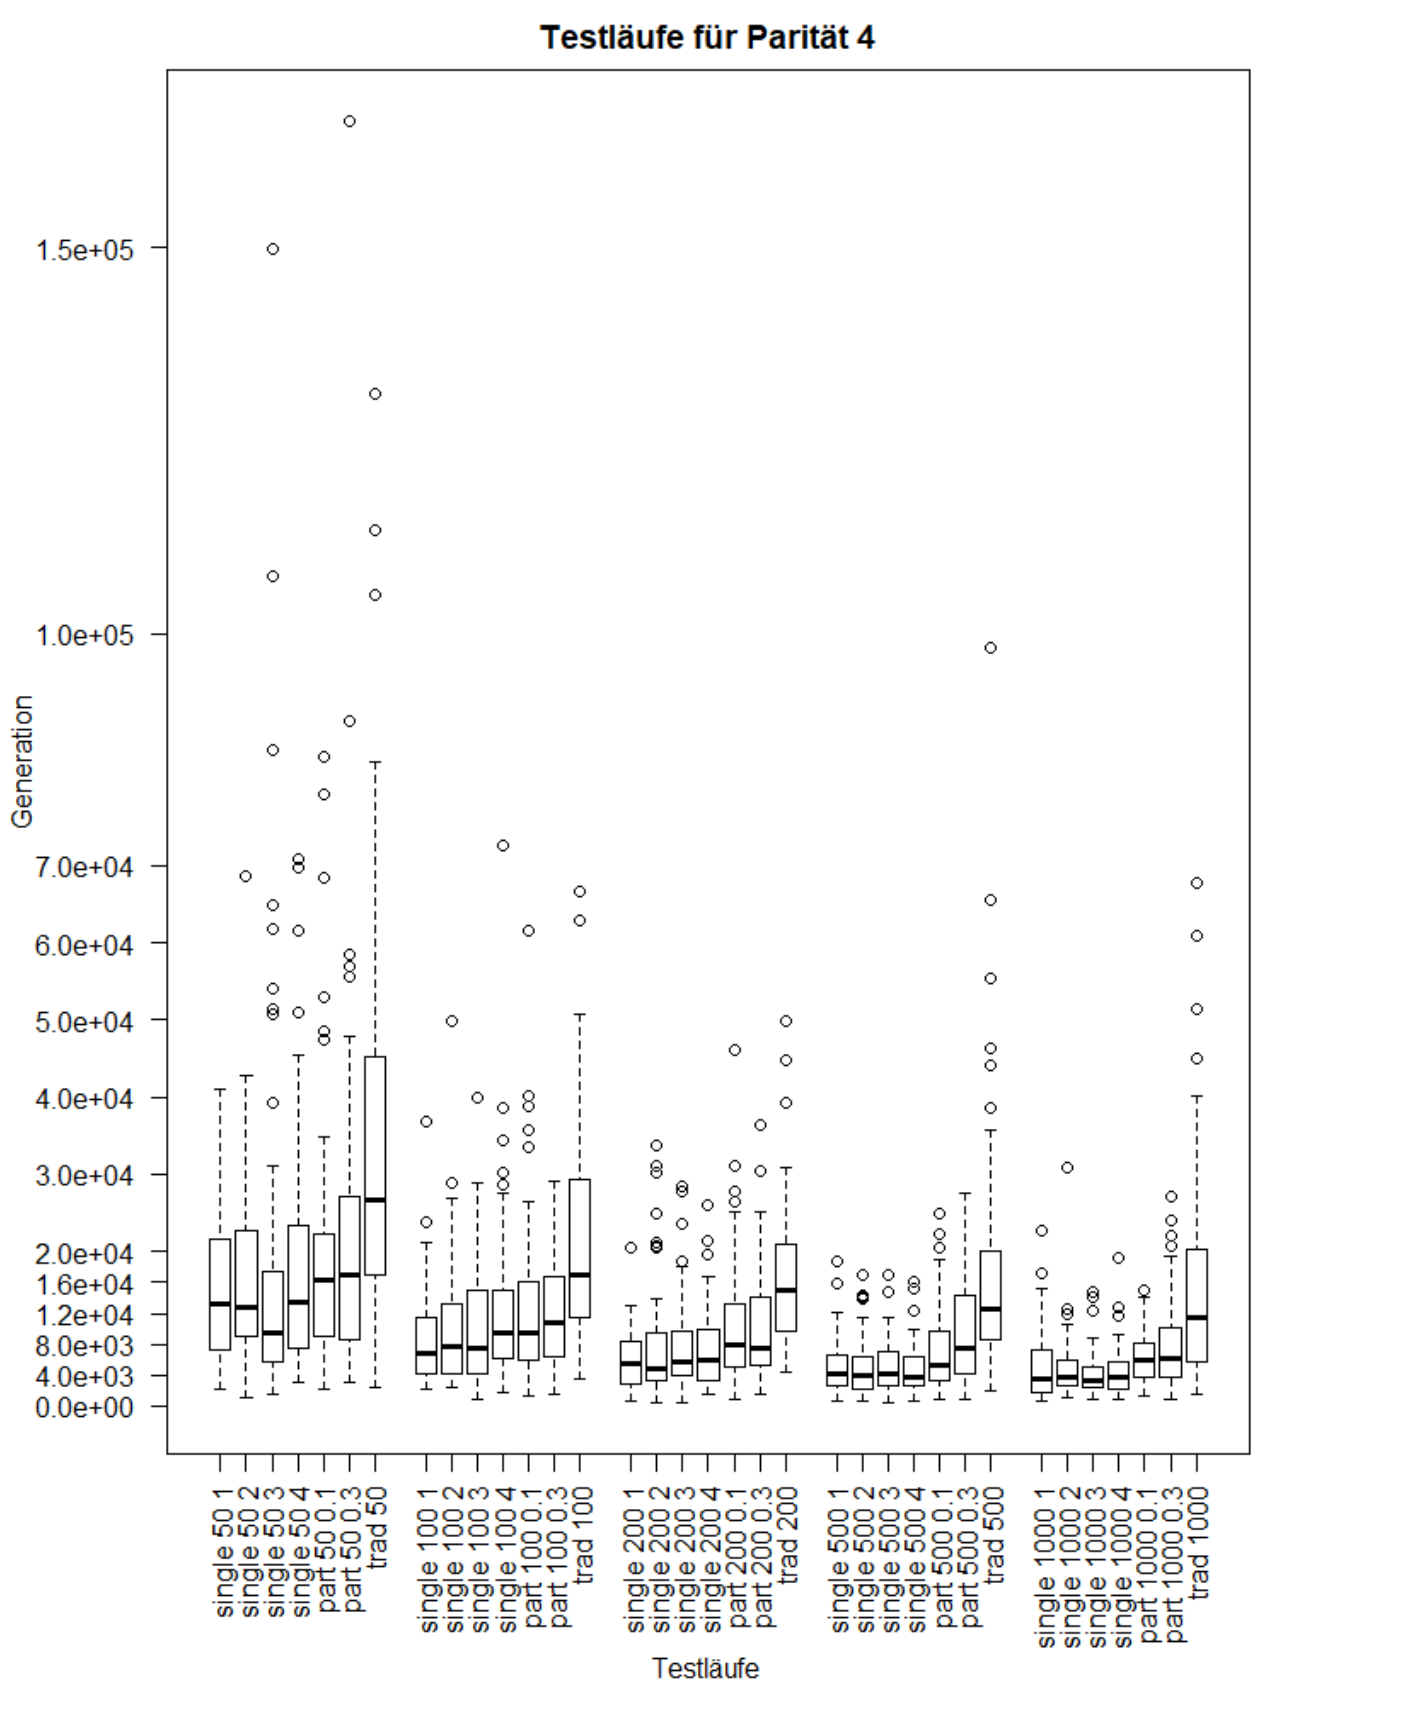
\includegraphics[scale=0.5]{parity4plotzoomed}
\caption[Testläufe Parität 4]{}
\end{figure}

\begin{figure}[h !]
\hspace*{-2.0cm}	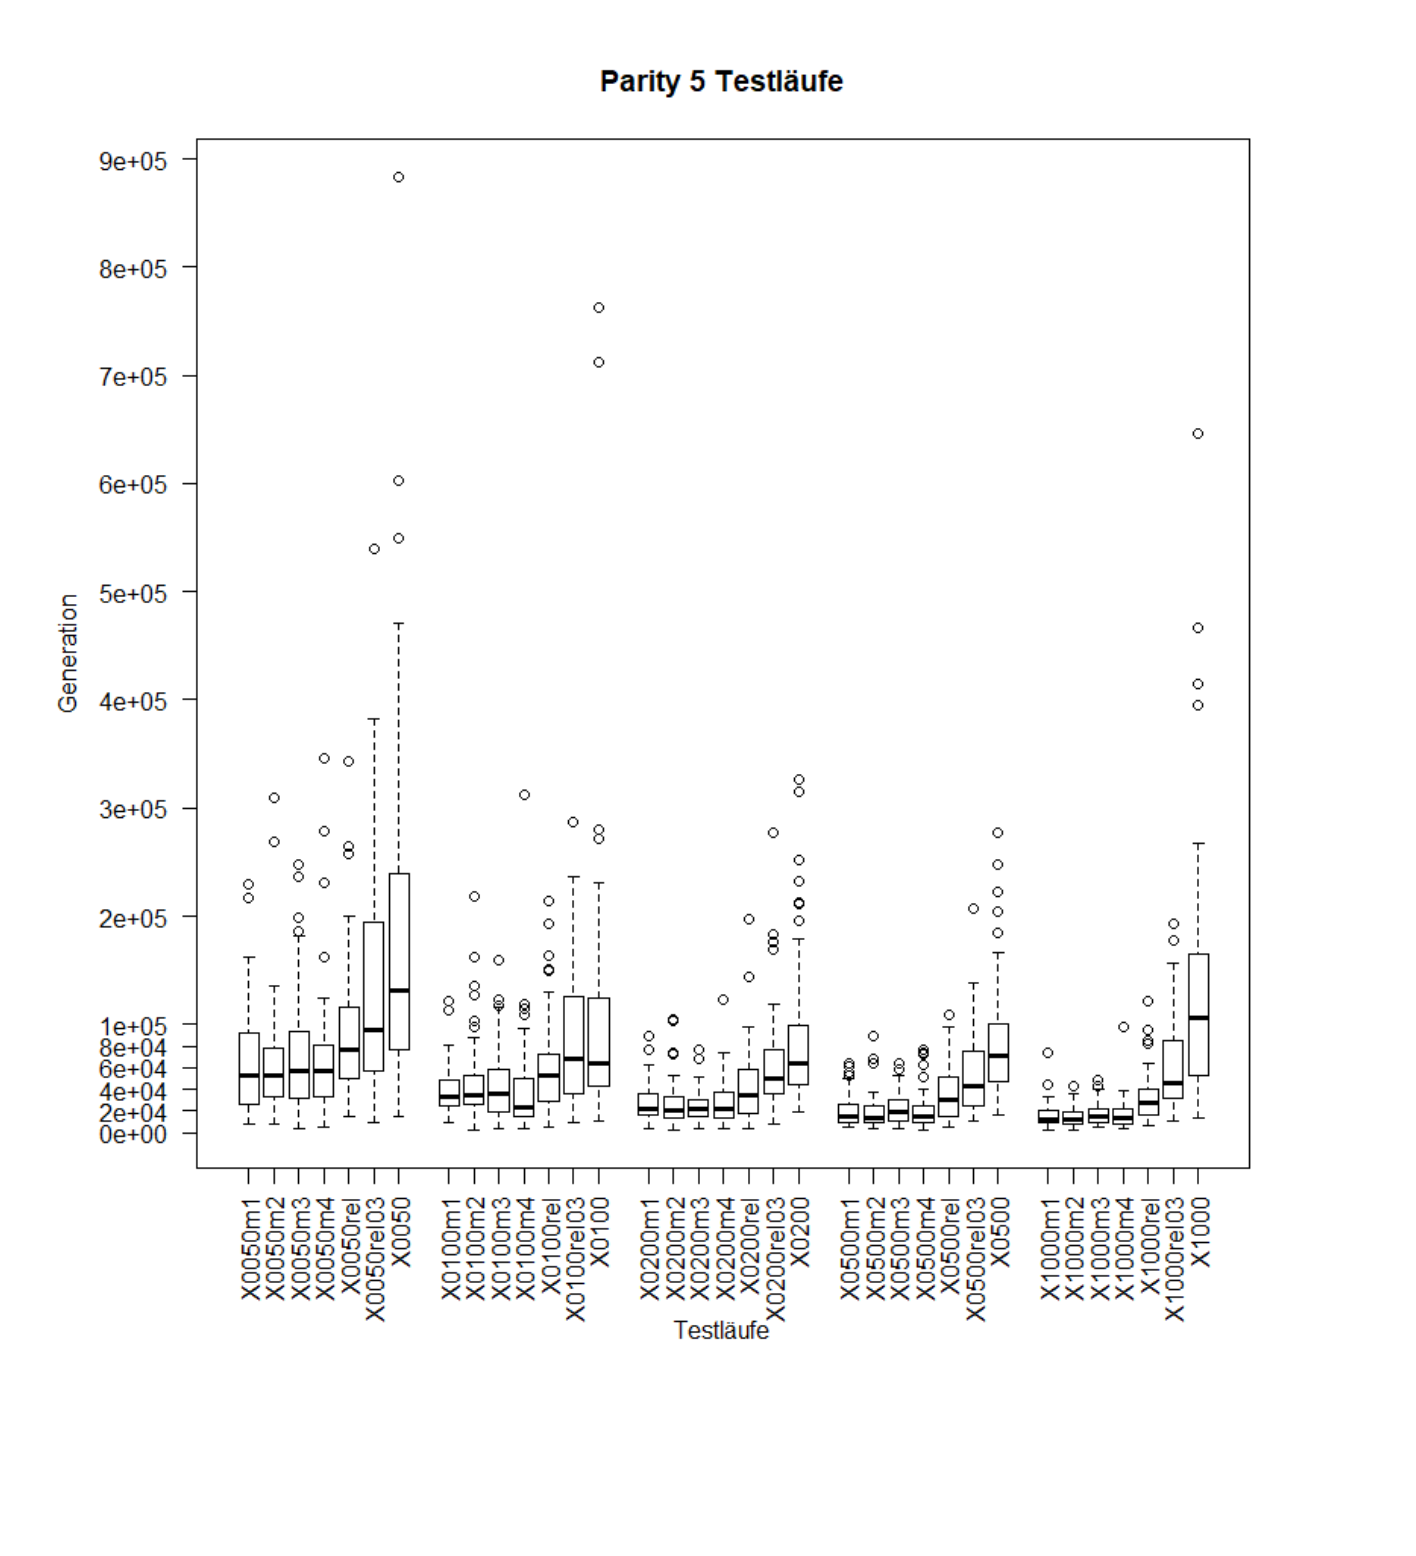
\includegraphics[scale=0.5]{parity5plotzoomed}
\caption[Testläufe Parität 5]{}
\end{figure}

\begin{figure}[h !]
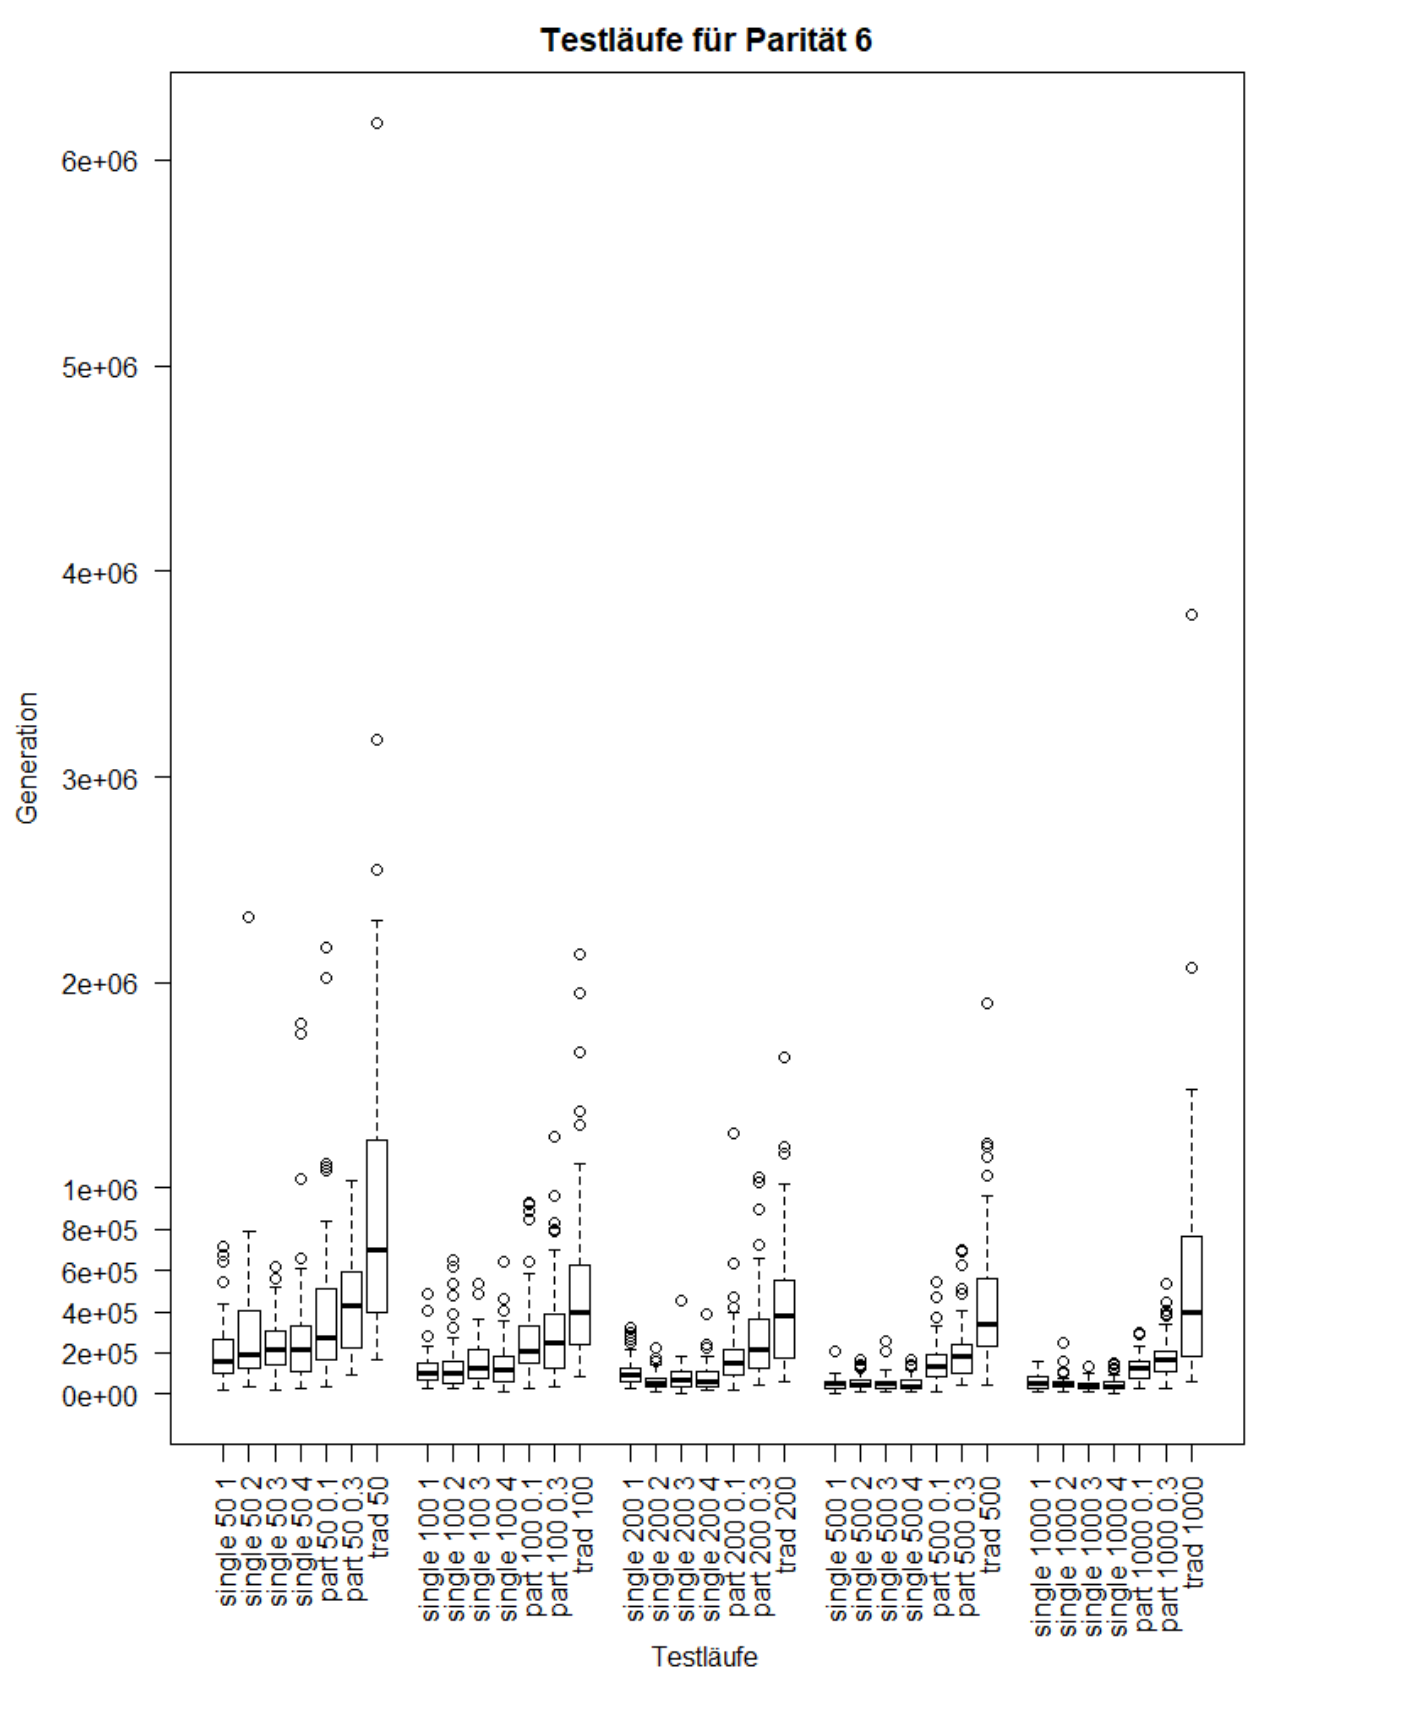
\includegraphics[scale=0.5]{parity6plotzoomed}
\caption[Testläufe Parität 6]{}
\end{figure}

\begin{figure}[h !]
\hspace*{-2.0cm}	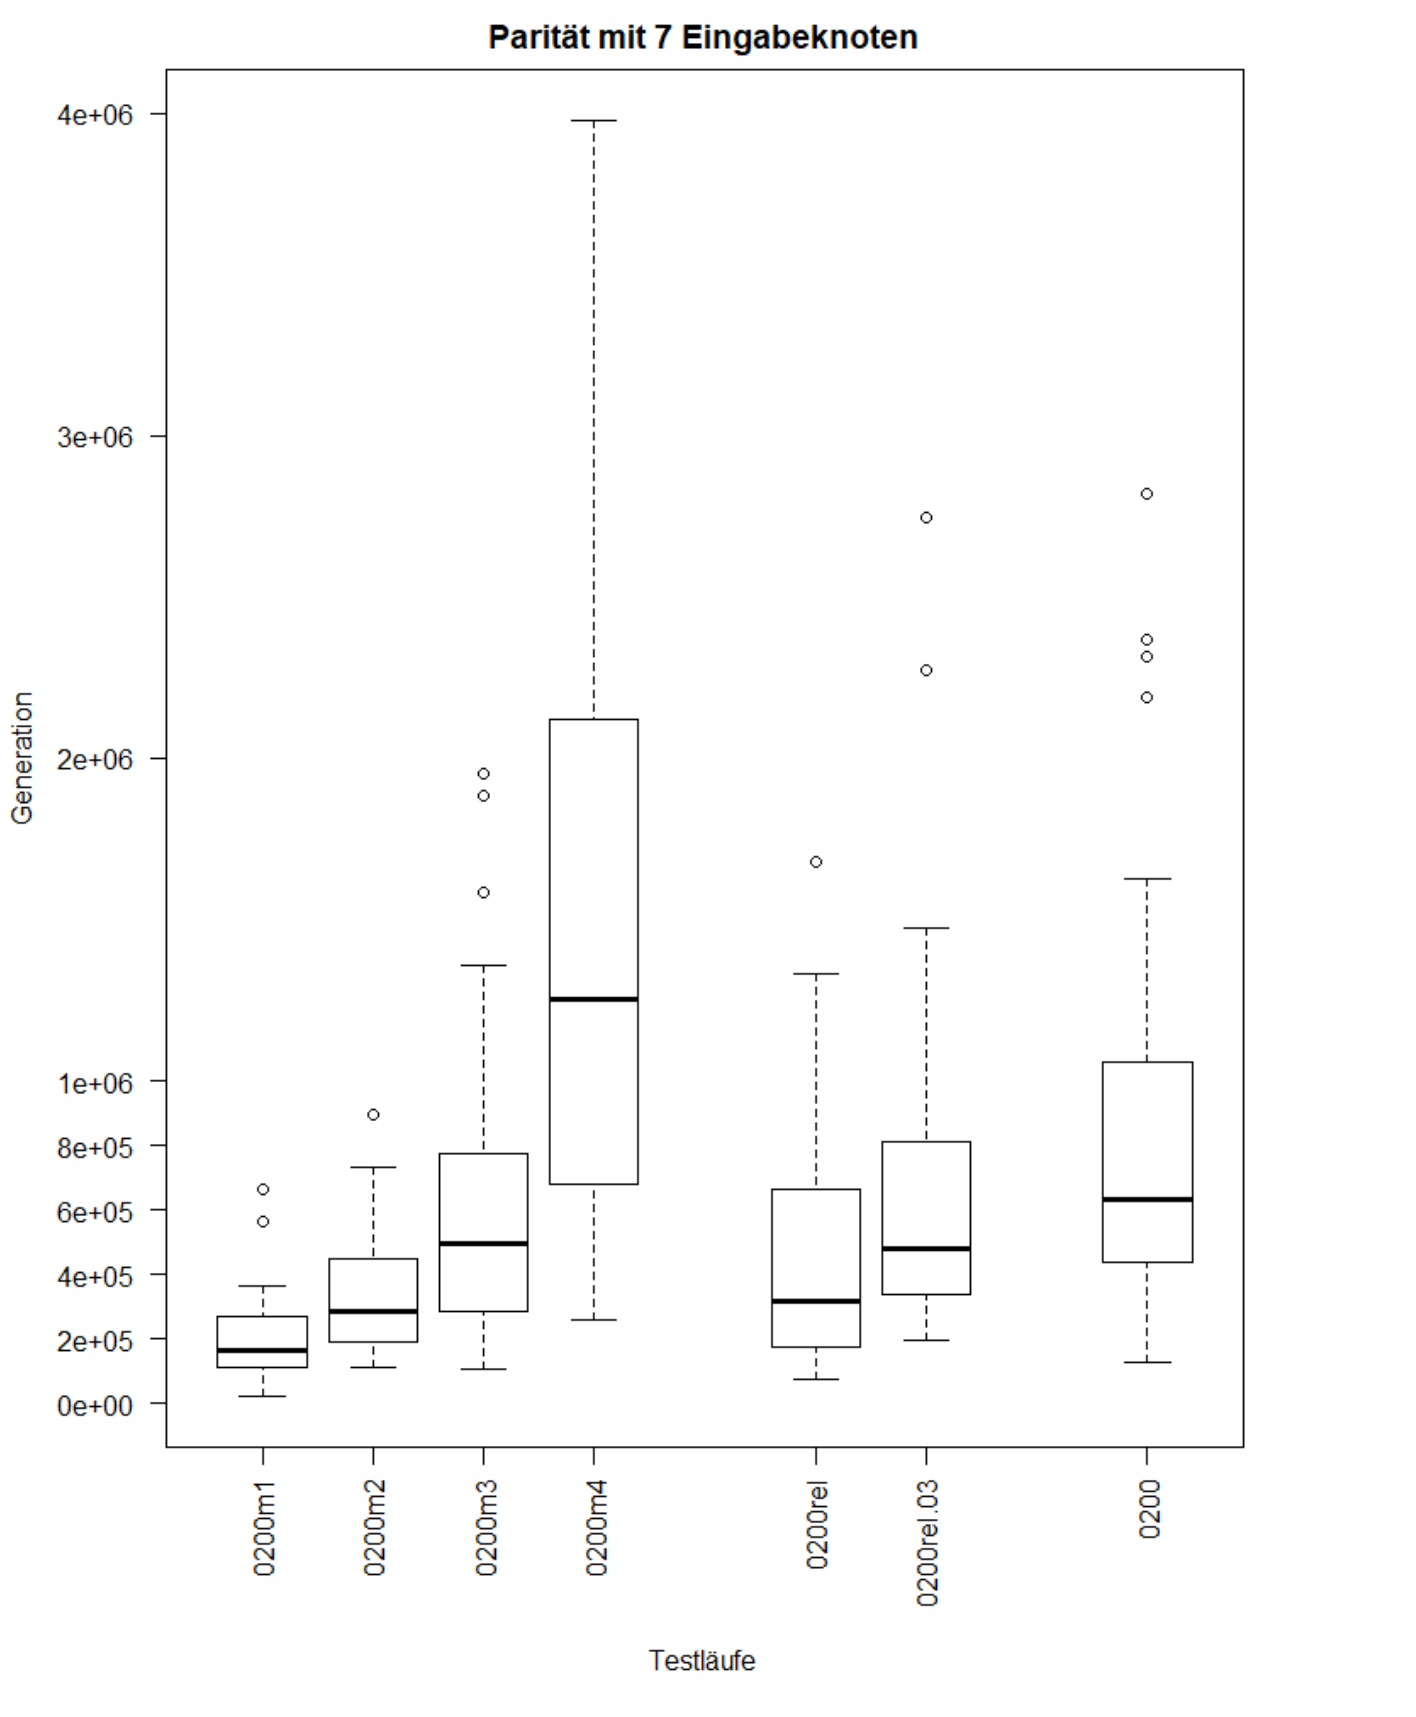
\includegraphics[scale=0.5]{parity7plotzoomed}
\caption[Testläufe Parität 7, 200 Knoten]{}
\end{figure}


\begin{figure}[h !]
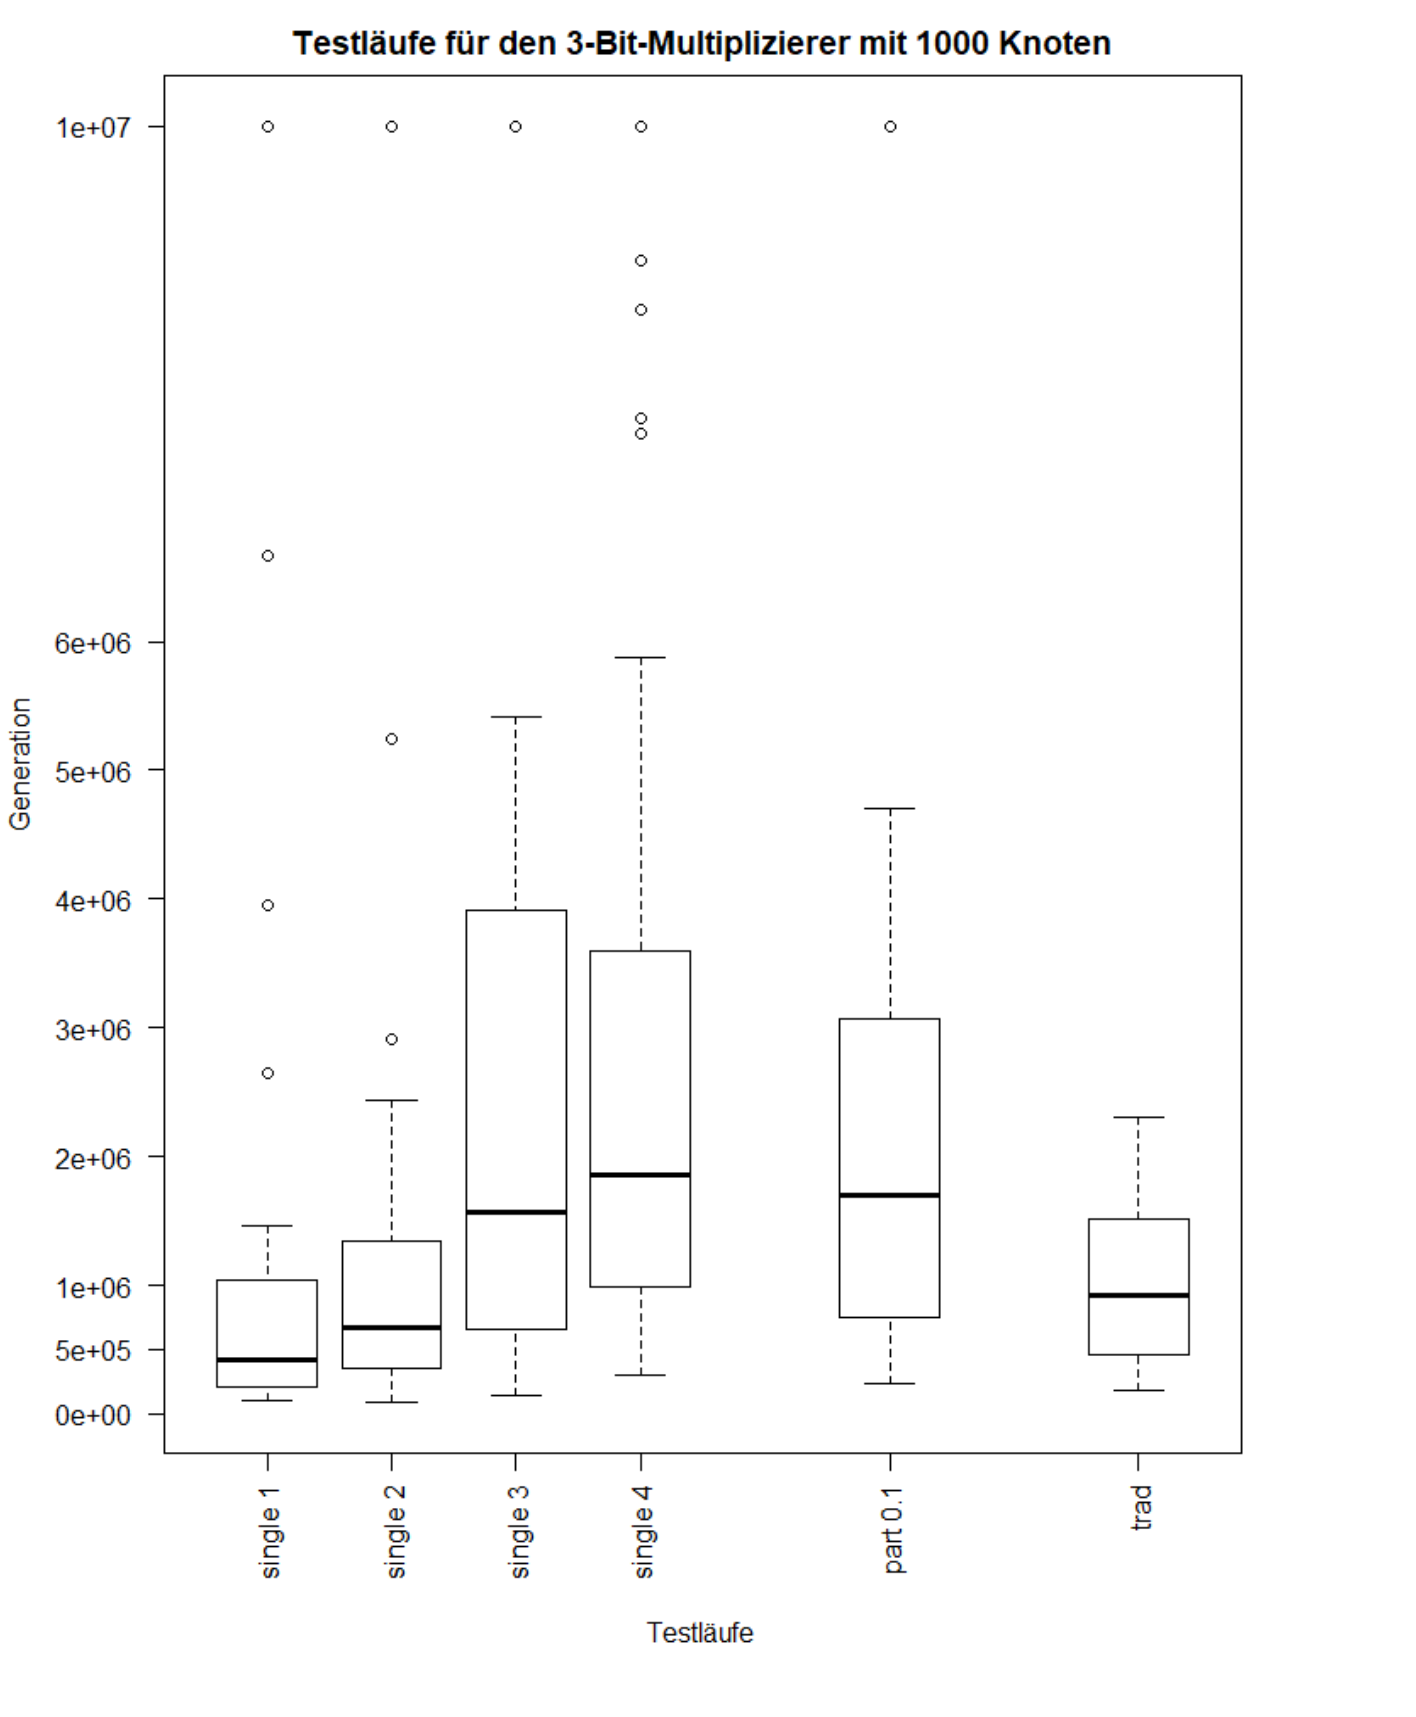
\includegraphics[scale=0.5]{mul3plotzoomed}
\caption[Testläufe 3-Bit-Multiplizierer, 1000 Knoten]{}
\end{figure}

\section{Diskussion}


die 'single active gene mutation' hat eindeutige Vorteile, beim lösen des Paritätsproblem bewiesen. Auch wenn anzunehmen ist, dass bei einem kleineren Graphen eine kleinere Mutationsrate effektiver ist, lies sich das für 'single active gene mutation' auf dem Paritätsproblem nicht erkennen (Bsp. Figur 2). Dies gilt jedoch nicht für das 3-Bit-Multiplizierer Problem, hier konnten viele Durchläufe nicht unter 10000000 Generationen zu einem angemessenen Ergebnis kommen. Hierbei war vor allem die Anzahl der Knoten im Graphen relevant, wobei erst ab 500 Knoten knapp zwei-drittel der Jobs und bei 1000 Knoten über 50 von 60 Jobs vor 10000000 Generationen beendet werden konnten. Somit war der traditionelle Algorithmus der einzige, welcher in jedem Job rechtzeitig beendet hat. Setzt man jedoch die fehlenden Durchläufe auf 10000000, so gibt es dennoch einige Konfigurationen, bei denen die 'single active gene mutation' besser abgeschnitten hat als der traditionelle Algorithmus. 

Dies ist besonders interessant, wenn man diesen Algorithmus mit dem aus 
\cite{conf/eurogp/GoldmanP13}
vergleicht, diese hatten einen ähnlichen Mutationsalgorithmus, welcher ebenfalls genau ein aktiven knoten mutiert hat, allerdings auch eine Mutationswahrscheinlichkeit genutzt hat um nicht aktive knoten zu mutieren. Bei ihnen war der traditionelle Algorithmus auf dem Paritätsproblem ungefähr gleich gut, teilweise sogar besser, allerdings war der traditionelle Algorithmus auf dem Multiplizierer Problem deutlich schlechter als ihre Variante der 'single active gene mutation'. 


die 'partial active gene mutation' hatte auf dem 3-Bit-Multiplizierer ähnliche Probleme wie die 'single active gene mutation', konnte jedoch bei den Paritätsproblemen nicht so gut abschneiden. Somit scheint die 'single active gene mutation' bei einer wachsenden Anzahl aktiver knoten kein problem damit zu haben, dass die Anzahl der Mutationen gleich bleibt, während die menge auf der mutiert wird potenziell steigt oder sinkt. Im Gegenteil scheint das sogar (zumindest bei dem Paritätsproblem) etwas gutes zu sein. 

\subsection{Analyse der Hypothese}

Das Resultat zeigt, dass 'single active gene mutation' dem traditionellen Mutationsalgorithmus nicht in allen Bereichen überlegen ist. Da die 'partial active gene mutation' für das Paritätsproblem besser als der traditionelle Algorithmus, bei beiden problem jedoch schlechter als 'single active gene mutation' funktionierte, ist naheliegend, dass 'single active gene mutation' kein problem mit einer fluktuierenden Menge aktive Knoten hat. 

Auffällig ist jedoch, dass trotz der nicht beendeten Durchläufe bei 1000 Knoten im Graphen die Versuche mit ;utationsraten von einem und zwei knoten genauso gut bzw. bessere Median und Quartile haben, wie der traditionelle Algorithmus. ein denkbarer Grund wäre, dass für das multiplizierer problem geringe Mutationsraten bessere erfolge bringen. Da die Idee hinter single active mutation ist, dass sich bei jeder Mutation der Phenotyp ändert, kann nicht weniger als ein aktiver knoten mutieren, wodurch die Mindestmutationsrate bei Graphen mit einer kleinen Anzahl knoten automatisch sehr hoch ist.


